\documentclass[tikz,border=10pt]{standalone}
\usepackage{tikz}
\usetikzlibrary{positioning}
\usepackage{tikz-feynman}
\begin{document}

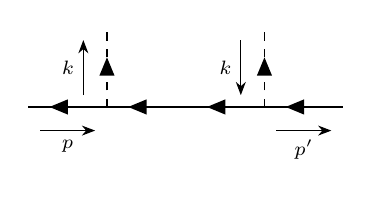
\begin{tikzpicture}
	\begin{feynman}
		%% fig a
		\vertex (a1) at (0,0);
		\vertex[right =1cm  of a1] (a2);
		\vertex[right =2cm  of a1] (a3);
		\vertex[right =3cm  of a1] (a4);
		\vertex[right =4cm  of a1] (a5);
        \vertex[above =1cm of a2] (a6);
        \vertex[above =1cm of a4] (a7);
		%\node[above =1.5cm  of a5] {$a$};
		\diagram*{
		{ [edge=anti fermion]
                (a1) --[momentum'={\scriptsize \(p\)}]  (a2),
                (a2) --  (a3),
                (a3) -- (a4),
                (a4) --[momentum'={\scriptsize \(p^{\prime}\)}]  (a5),
		    },
            % 介子连线
        { [edge= charged scalar]
        (a2) --[momentum={\scriptsize \(k\)}](a6), 
        (a4) --[reversed momentum={\scriptsize \(k\)}](a7), 
		}
        };
	\end{feynman}
\end{tikzpicture}


\end{document}